\section{Guarantees and their scope}
\label{app:guarantees}
For completeness, the fixed-bank expectation bound in Equation~\eqref{eq:optimism} follows from a bounded-score argument. Write $M_j=\hat\theta_{Sj}$. Since $M_{\hat j}=\max_jM_j$,
\begin{align}
\mathbb{E}(M_{\hat j}-\theta_{\hat j})
&=\mathbb{E}\max_jM_j-\mathbb{E}\theta_{\hat j}\\
&\geq\max_j\theta_j-\mathbb{E}\theta_{\hat j}\geq0.
\end{align}
For $\lambda>0$, iid bounded observations imply
$\mathbb{E}e^{\lambda(M_j-\theta_j)}\leq e^{\lambda^2/(8n)}$. Therefore
\begin{align}
\mathbb{E}(M_{\hat j}-\theta_{\hat j})
&\leq\mathbb{E}\max_j(M_j-\theta_j)\\
&\leq\frac{\log K}{\lambda}+\frac{\lambda}{8n}.
\end{align}
Optimizing $\lambda$ yields the upper bound for $K>1$; for $K=1$ unbiasedness is immediate. Independence across configurations is unnecessary, while independence across question rows and a fixed family are essential to this argument.

If $C_j$ is a CP interval with marginal error $\alpha/K$, then
\begin{equation}
\Pr(\forall j:\theta_j\in C_j)\geq1-\sum_j\alpha/K=1-\alpha.
\end{equation}
Thus $\Pr(\theta_{\hat j}\in C_{\hat j})\geq1-\alpha$ for any selector within the protected family. On this simultaneous event, the winner cannot have a lower interval endpoint exceeding the default's upper endpoint when its true accuracy is no greater than the default's. This protects the specified simultaneous-interval comparison. It does not make the reused point estimate unbiased.

For a fresh independent audit of a frozen winner, conditional on the entire search dataset and its randomization, the audit count is $\mathrm{Binomial}(h,\theta_{\hat j})$. Conditional unbiasedness and CP coverage follow, and remain valid on averaging over search. The simple proof ceases to apply if audit outcomes guide further configuration changes. For a finite scored cache, iid resampling with replacement gives a conditional empirical-population target; that target is not automatically the unknown superpopulation accuracy. Our synthetic experiments use genuinely known Bernoulli parameters.

\section{Decision errors under selection}
\label{app:decisions}
\begin{figure*}[ht]
\centering
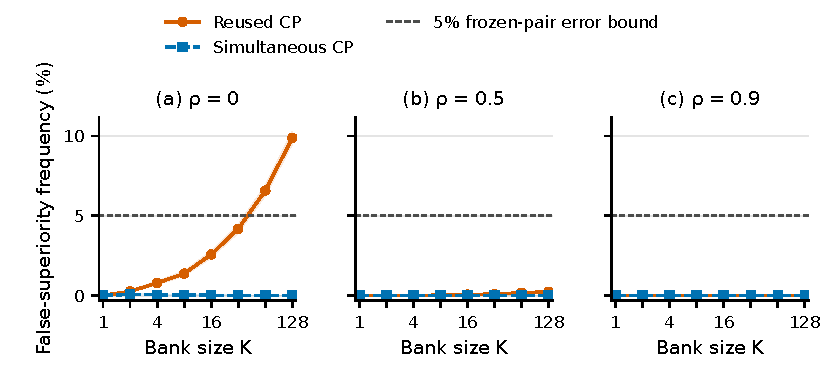
\includegraphics[width=\textwidth]{figures/synthetic-decisions.pdf}
\caption{\textbf{A conservative frozen-pair rule can become unreliable after winner selection.} At $n=512$, every candidate has accuracy 0.4. An event occurs when a selected nondefault winner's lower ordinary 95\% CP endpoint exceeds the default's upper endpoint. Rates are unconditional over all repetitions, not conditional false-discovery rates. The dashed 5\% line is the frozen-pair bound before selection. Simultaneous CP uses per-candidate error $0.05/K$. Columns vary equal-quality correlation $\rho$; bands are marginal exact 95\% binomial Monte Carlo intervals over 20,000 repetitions. At $\rho=0$, $K=128$, the ordinary-rule rate is 9.89\% (MCSE 0.211 pp). Zero events would not establish zero population risk. This rule is not a paired test.}
\end{figure*}

\section{Complete synthetic grid}
\label{app:fullgrid}
\begin{figure*}[ht]
\centering
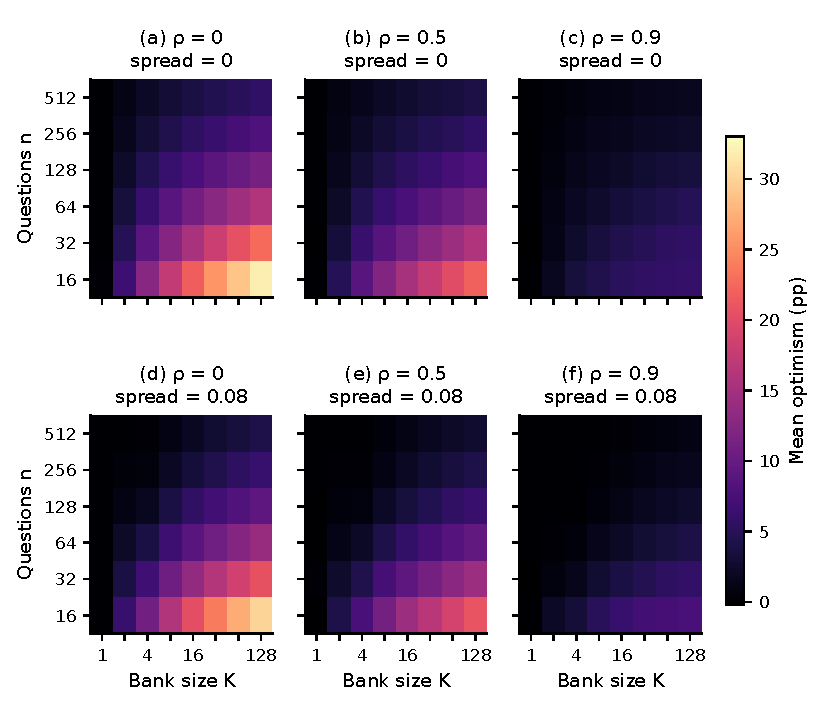
\includegraphics[width=\textwidth]{figures/synthetic-optimism-grid.pdf}
\caption{\textbf{Reused-score optimism in all 288 settings.} Color is mean winning search accuracy minus selected true accuracy, in percentage points. Rows vary quality spread, columns the shared-question mixture probability $\rho$; each panel crosses $n$ and $K$. At spread zero all accuracies are 0.4. At spread 0.08, nondefault means range over $[0.32,0.48]$; $K=2$ has a single 0.48 challenger, and $K=1$ only the default. Thus $K$ also changes the quality grid in heterogeneous cells. With unequal means $\rho$ is not exactly pairwise correctness correlation. The minimum estimate is $-0.176$ pp, reflecting Monte Carlo variation despite nonnegative expected optimism in this model. Complete per-cell MCSEs and seeds accompany the input CSV; this is not simultaneous inference about extrema.}
\end{figure*}
\begin{figure*}[ht]
\centering
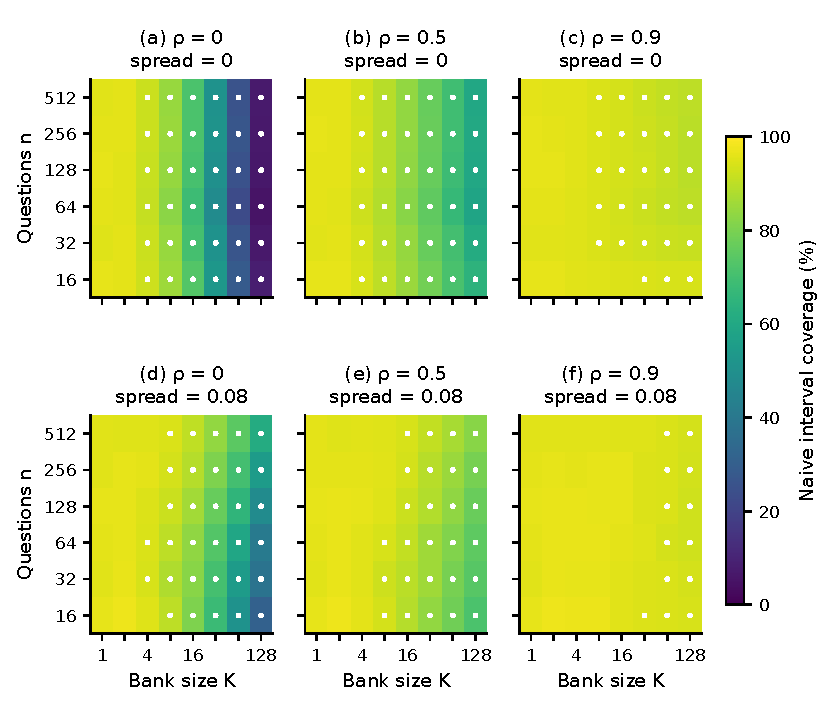
\includegraphics[width=\textwidth]{figures/synthetic-coverage-grid.pdf}
\caption{\textbf{Naive selected-target coverage in all 288 settings.} Settings match the optimism grid; color is the fraction of 20,000 repetitions where the ordinary nominal 95\% CP interval contains the selected candidate's known accuracy. A white dot marks a cell whose marginal exact 95\% Monte Carlo upper limit is below 95\%; these diagnostics are uncorrected across cells. Absence of a dot is not evidence of guaranteed coverage. Means, MCSEs, and seeds are retained in the complete source CSV.}
\end{figure*}

\section{Point-estimation error}
\label{app:mse}
\begin{figure*}[ht]
\centering
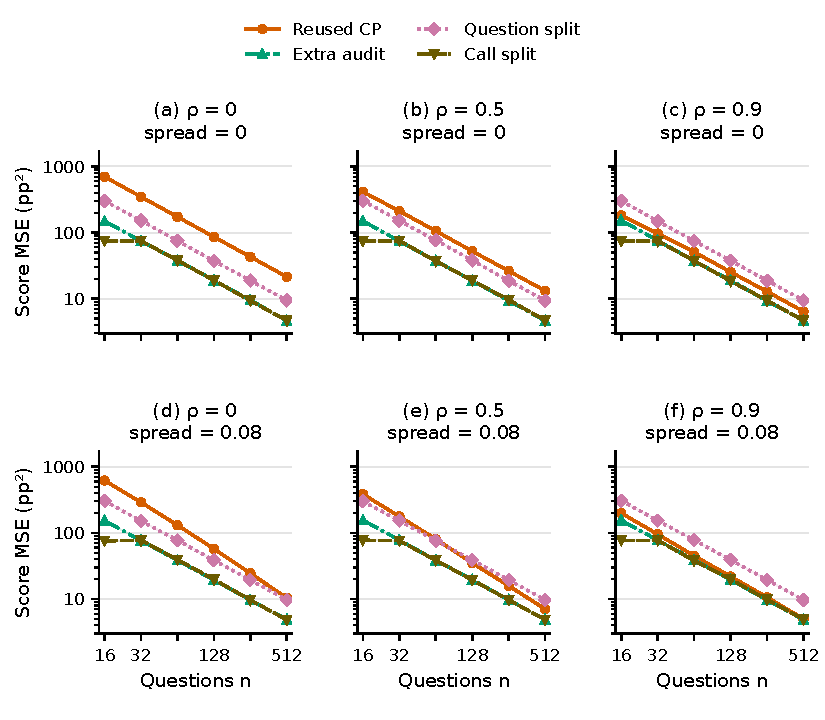
\includegraphics[width=\textwidth]{figures/synthetic-mse.pdf}
\caption{\textbf{MSE depends on protocol, resources, and candidate dependence.} At $K=32$, MSE averages squared error of a protocol's report relative to its selected true accuracy, in squared percentage points (log scale). Rows vary spread, columns shared-question mixture probability. Candidate means and resource definitions match the main figures. Simultaneous CP is omitted because it preserves the reused score and has identical MSE. Bands are mean $\pm1.96$ MCSE on the untransformed scale. Extra audit adds $n$ calls; question and call splits change selection resources and can select different configurations. These outcomes do not establish universal dominance or an actual LLM population effect.}
\end{figure*}

\section{Synthetic reproduction and compute}
The full grid was generated by \texttt{scripts/run\_synthetic.py} in the analysis package with \texttt{--reps 20000}, master seed 20261103, and independent cell seeds recorded in every output row. The exact-null reference script and distributional checks are delivered separately from the plotting code. Every synthetic figure and Table~\ref{tab:methods} is generated by \texttt{presentation/render.py} from hash-checked committed analysis inputs. The generator performs no simulation; it preserves upstream seeds and checks completeness and uniqueness of the metric grid. Each point-estimation band is mean $\pm1.96$ MCSE; event-rate bands use marginal exact binomial intervals, including nonzero upper limits for zero events.

The main synthetic run took 89.8811 measured computational wall seconds and 89.7073 process CPU seconds, with peak resident memory 285,564 KB. These timers exclude interpreter/import startup. The three-cell, 1,000-repetition pilot took 0.1761 wall seconds and 0.1614 process CPU seconds; its preliminary values are not substituted for full-grid results. No full-grid cells failed or were omitted. Plotting is documented separately by the presentation owner. The delivered reproduction instructions must also account for inference setup attempts and actual real-model generation; simulation timings are not total study costs.
